\chapter{Исследование влияние параметров осаждения верхнего электрода на микроскопические свойства структур W/HZO/Pt}

\section{Изготовление структур}

Для исследования были изготовлены 4 образца: на кремниевой подложке методом магнетронного напыления формировался вольфрам толщиной \SI{40}{\nm}, далее методом атомно-слоевого осаждения выращивался оксид гафния-циркония толщиной \SI{10}{\nm} и затем методом импульсного лазерного напыления осаждалась платина. При этом в качестве параметра при изготовлении структур варьировалась энергия импульса, используемого при импульсном лазерном напылении (в дальнейшем "--- энергия импульса). Чтобы обеспечить качество электрического контакта, по центру структур методом электронно-лучевого напыления были сформированы алюминиевые пады. Схематическое изображение структур (вид сбоку) представлено на рис. \cref{sample_structure}, изображения изготовленных образцов, полученные с помощью оптического микроскопа (вид сверху), представлены на рис. \cref{sample_optics}.

\begin{figure}[ht]
    \centerfloat{
        \hfill
        \subcaptionbox[List-of-Figures entry]{\label{sample_structure} Схематическое изображение структур}{%
            \includegraphics[width=0.5\linewidth]{sample_structure.png}}
        \hfill
        \subcaptionbox{\label{sample_optics} Изображение структур в оптическом микроскопе}{%
            \includegraphics[width=0.5\linewidth]{sample_optics.png}}
        \hfill
    }
    \caption[Этот текст попадает в названия рисунков в списке рисунков]{Изображения исследуемых структур}
\end{figure}

\section{Исследование морфологии}

\subsection{Морфология поверхности Pt}

Для изучения свойств поверхности была исследована морфология поверхности Pt. Для получения значений шероховатости и толщины плёнок использовалась АСМ (рис. \cref{fig:afm:morphology}), а для получения значений размера зёрен "--- растровая электронная микроскопия (РЭМ) (\cref{fig:sem:morphology}) \todo{добавить чуть-чуть про РЭМ, XRD в методы}. Выбор РЭМ для исследования размера зёрен обусловлен более высоким пространственным разрешением прибора по сравнению с АСМ. Основные результаты сведены в таблицу \cref{tab:morphology_pt}.
\begin{figure}[ht]
    \centerfloat{
        \hfill
        \subcaptionbox[List-of-Figures entry]{\label{fig:afm:morphology:45mJ} \SI{45}{\milli\joule}}{%
            \includegraphics[width=0.5\linewidth]{afm/morphology/45 mJ.png}}
        \hfill
        \subcaptionbox{\label{fig:afm:morphology:93mJ} \SI{93}{\milli\joule}}{%
            \includegraphics[width=0.5\linewidth]{afm/morphology/93 mJ.png}}
        \hfill
        \\
        \subcaptionbox{\label{fig:afm:morphology:145mJ} \SI{145}{\milli\joule}}{%
            \includegraphics[width=0.5\linewidth]{afm/morphology/145 mJ.png}}
        \hfill
        \subcaptionbox{\label{fig:afm:morphology:225mJ} \SI{225}{\milli\joule}}{%
            \includegraphics[width=0.5\linewidth]{afm/morphology/225 mJ.png}}
        \hfill
    }
    \caption[Этот текст попадает в названия рисунков в списке рисунков]{Морфология поверхности плёнки платины при различных энергиях импульса (АСМ)}\label{fig:afm:morphology}
\end{figure}

\begin{figure}[ht]
    \centerfloat{
        \hfill
        \subcaptionbox[List-of-Figures entry]{\label{fig:sem:45mJ} \SI{45}{\milli\joule}}{%
            \includegraphics[width=0.48\linewidth]{sem/45 mJ.png}}
        \hfill
        \subcaptionbox{\label{fig:sem:93mJ} \SI{93}{\milli\joule}}{%
            \includegraphics[width=0.5\linewidth]{sem/93 mJ.png}}
        \hfill
        \\
        \subcaptionbox{\label{fig:sem:145mJ} \SI{145}{\milli\joule}}{%
            \includegraphics[width=0.51\linewidth]{sem/145 mJ.png}}
        \hfill
        \subcaptionbox{\label{fig:sem:225mJ} \SI{225}{\milli\joule}}{%
            \includegraphics[width=0.5\linewidth]{sem/225 mJ.png}}
        \hfill
    }
    \caption[Этот текст попадает в названия рисунков в списке рисунков]{Морфология поверхности плёнки платины при различных энергиях импульса (РЭМ)}\label{fig:sem:morphology}
\end{figure}

\begin{table} [htbp]
    \centering
    \begin{threeparttable}% выравнивание подписи по границам таблицы
        \caption{Характеристики плёнки Pt}\label{tab:morphology_pt}%
        \begin{tabular}{  | p{3.7cm}  | p{2.4cm}| p{2.7cm} | p{3.6cm}l | }
            \hline
            \hline
            \centering Энергия импульса, \si{\milli\joule} & \centering Толщина, \si{\nm} & \centering Шерохова\-тость, \si{\nm} & \centering Средний размер зёрен, \si{\nm} & \\
            \hline
            \centering 225                                 & \centering  30-40            & \centering 0.90                      & \centering 20                             & \\
            \centering 145                                 & \centering 28-37             & \centering 0.59                      & \centering 32                             & \\
            \centering 93                                  & \centering 14-20             & \centering 0.37                      & \centering 45                             & \\
            \centering 45                                  & \centering 3-7               & \centering 0.45                      & \centering 100                            & \\
            \hline
            \hline
        \end{tabular}
    \end{threeparttable}
\end{table}

\todo{Прежде всего стоит отметить явную зависимость толщины плёнки от энергии импульса, использованного при напылении. Вероятно, это объясняется постоянным временем напыления (т.е. одинаковым количеством импульсов) при различной энергии одиночного импульса. Таким образом, при более энергичном излучении платина распыляется интенсивнее, формируя более толстую плёнку.}

Из полученных изображений и из результатов их анализа также заметно увеличение размера зёрен и шероховатости плёнок при увеличении энергии импульса. \todo{Для получения распределения размера зёрен платины была проведена обработка снимков РЭМ с помощью алгоритма watershed, также подтверждающая увеличение размера зёрен (рис. 4). Если будешь добавлять распределения, переформулируй прошлое предложение (из полученных изображений), а про анализ вставь сюда}

\newpage
\subsection{Морфология HZO}

Анализ изображений плёнки HZO показал отсутствие явной зависимости размера зёрен от энергии импульса (рис. \cref{fig:sem:hzo_grains}, табл. \cref{tab:morphology_hzo}).

\begin{figure}[ht]
    \centerfloat{
        \hfill
        \subcaptionbox[List-of-Figures entry]{\label{fig:sem:hzo_grains_probability} Распределение зёрен по вероятности}{%
            \includegraphics[width=0.49\linewidth]{sem/hzo_grains_probability.jpg}}
        \hfill
        \subcaptionbox{\label{fig:sem:hzo_grains_area} Распределение зёрен по занимаемой площади}{%
            \includegraphics[width=0.49\linewidth]{sem/hzo_grains_area.jpg}}
        \hfill
    }
    \caption[Этот текст попадает в названия рисунков в списке рисунков]{Характеристики зёрен HZO}\label{fig:sem:hzo_grains}
\end{figure}

\begin{table} [htbp]
    \centering
    \begin{threeparttable}% выравнивание подписи по границам таблицы
        \caption{Характеристики плёнки HZO}\label{tab:morphology_hzo}%
        \begin{tabular}{  | p{3.5cm}  | p{5.7cm}| p{6.2cm}l | }
            \hline
            \hline
            \centering Энергия импульса, \si{\milli\joule} & \centering Размер наиболее встречающихся зёрен, \si{\nm} & \centering Размер зёрен, занимающих наибольшую площадь, \si{\nm} & \\
            \hline
            \centering 225                                 & \centering 25                                            & \centering 56                                                    & \\
            \centering 145                                 & \centering 22                                            & \centering 40                                                    & \\
            \centering 93                                  & \centering 27                                            & \centering 43                                                    & \\
            \centering 45                                  & \centering 28                                            & \centering 48                                                    & \\
            \hline
            \hline
        \end{tabular}
    \end{threeparttable}
\end{table}

\section{Исследование доменной структуры}

Поскольку результаты АСМ и электрофизические измерения показывают монотонную динамику влияния энергии импульса на свойства образцов, измерения методом микроскопии пьезоотклика проводились лишь на образцах с наименьшей (\SI{45}{\milli\joule}) и наибольшей (\SI{225}{\milli\joule}) энергиями импульса.

\subsection{Динамика переключений}

Результаты исследования изменения доменной структуры во время циклирования приведены на рисунке \cref{fig:pfm:wake-up}. В ходе циклирования образца с энергией импульса \SI{45}{\milli\joule} (рис. \cref{fig:pfm:wake-up:45mJ}) заметно плавное увеличение области, которую занимают переключающиеся домены, что, вероятно, связано с постепенным уменьшением встроенного поля, приводящим к депиннингу доменов \todo{ref}. Кроме того, наблюдается корреляция доли переключаемых доменов с величиной остаточной поляризации, полученной при циклировании аналогичной структуры при электрофизических измерениях. В образце с энергией импульса \SI{225}{\milli\joule} (рис. \cref{fig:pfm:wake-up:225mJ}) сегнетоэлектрическая плёнка переключается полностью после первого же импульса.

\begin{figure}[ht]
    \centerfloat{
        \subcaptionbox[List-of-Figures entry]{\label{fig:pfm:wake-up:45mJ} Энергия импульса 45 мДж}{%
            \includegraphics[width=0.8\linewidth]{pfm/wake-up/45 mJ.png}}
        \\
        \hfill
        \subcaptionbox{\label{fig:pfm:wake-up:225mJ} Энергия импульса 225 мДж}{%
            \includegraphics[width=0.53\linewidth]{pfm/wake-up/225 mJ.png}}
    }
    \caption[Этот текст попадает в названия рисунков в списке рисунков]{Динамика переключений при различных энергиях импульса}\label{fig:pfm:wake-up}
\end{figure}

\subsection{Полидоменное состояние}

Исследование полидоменного состояния было проведено с помощью подачи импульсов с различным напряжением на проциклированную структуру. При этом также наблюдалась корреляция остаточной поляризации и доли переключающихся доменов, теперь уже в зависимости от амплитуды прикладываемого импульса \cref{fig:pfm:polydomain:hyst}. Обе плёнки полностью переключаются при напряжениях \(\sim\) \SI{4}{\volt}, что свидетельствует о почти полном отсутствии зёрен неполярной (тетрагональной или моноклинной) фазы в составе сегнетоэлектрической плёнки, что также подтверждается результатами рентгеновской дифракции для образца с меньшей энергией импульса (рис. \cref{fig:xrd}).


\begin{figure}[ht]
    \centerfloat{
        \subcaptionbox[List-of-Figures entry]{\label{fig:pfm:polydomain:pv_hyst} Поляризация в зависимости от поданного напряжения (\(PV\)-гистерезис)}{%
            \includegraphics[width=0.49\linewidth]{pfm/polydomain/pv_hysteresis.png}}
        \hfill
        \subcaptionbox{\label{fig:pfm:polydomain:domain_hyst} Доля переключённых доменов в зависимости от напряжения переключающего импульса}{%
            \includegraphics[width=0.49\linewidth]{pfm/polydomain/domain_hysteresis.png}}
    }
    \caption[Этот текст попадает в названия рисунков в списке рисунков]{Динамика переключений при различных амплитудах переключающего импульса}\label{fig:pfm:polydomain:hyst}
\end{figure}

\begin{figure}[ht]
    \centerfloat{
        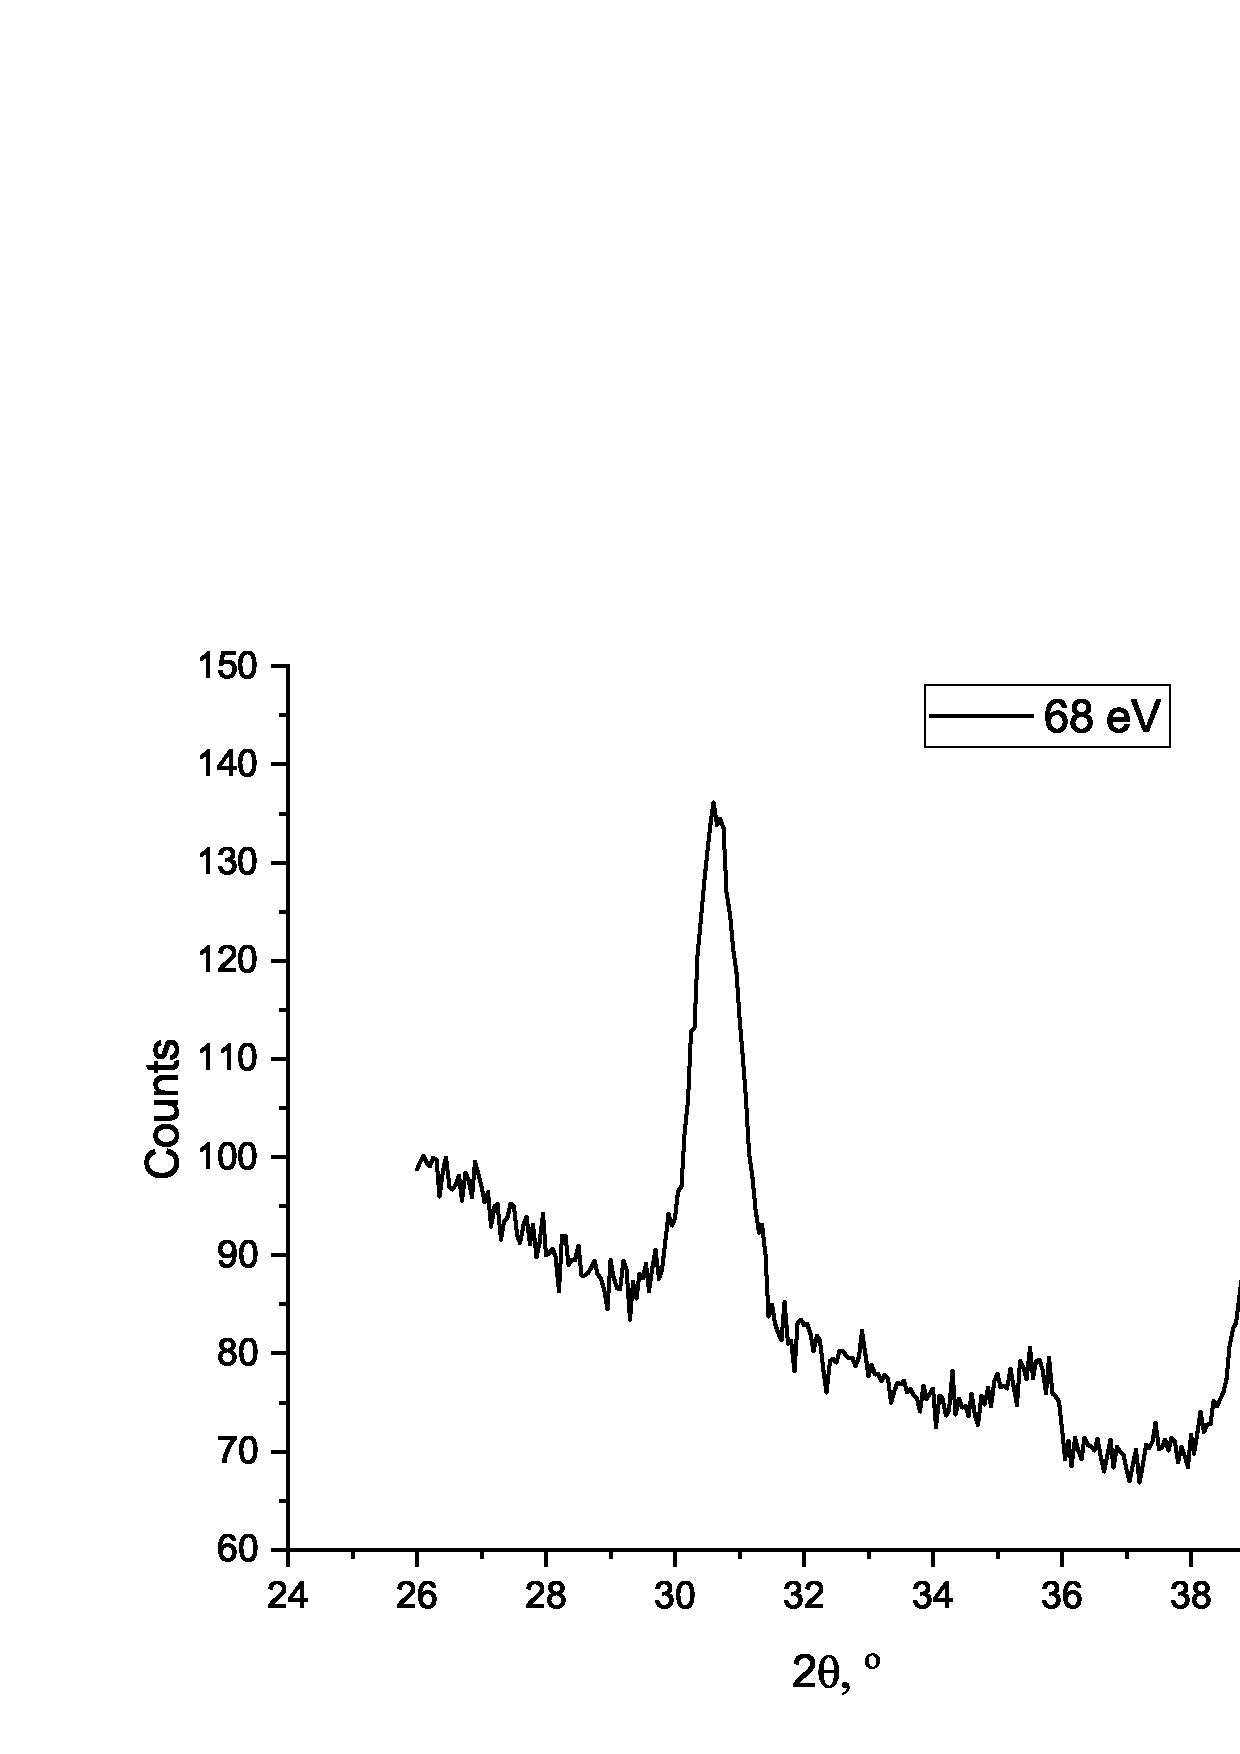
\includegraphics[scale=0.5]{xrd.png}
    }
    \caption{Дифрактограмма HZO в образце с меньшей энергией импульса}\label{fig:xrd}
\end{figure}

Далее на конденсаторы были поданы импульсы с напряжением порядка коэрцитивного для переключения плёнки HZO в состояние с примерно одинаковой долей доменов в каждом из состояний (рис. \cref{fig:pfm:polydomain}). Было обнаружено, что при увеличении энергии импульса, использованного при напылении, увеличивается характерный размер доменов. Также можно заметить более чёткую доменную структуру образца с меньшей энергией. Данный факт можно объяснить более тонкой плёнкой платины, приводящей к более высокому разрешению доменной структуры при измерениях.

\begin{figure}[ht]
    \centerfloat{
        \includegraphics[scale=0.8]{pfm/polydomain/polydomain.png}
    }
    \caption{Карты фазы пьезоотклика в полидоменном состоянии}\label{fig:pfm:polydomain}
\end{figure}



\subsection{Латеральный пьезоотклик}

Для калибровки латерального отклика, описанной в разделе \cref{sec:ch2/sect1/sub1}, была использована структура TiN/HfO\(_2\)/TiN с участками СЭ HfO\(_2\):Ga \cite{chouprikNanoscaleTailoringFerroelectricity2020}. Полученные карты вертикального и латерального откликов показаны на рис. \cref{fig:pfm:lateral:calibration:vertical} и \cref{fig:pfm:lateral:calibration:lateral}.

\begin{figure}[ht]
    \centerfloat{
        \hfill
        \subcaptionbox[List-of-Figures entry]{\label{fig:pfm:lateral:calibration:vertical} Вертикальный отклик}{%
            \includegraphics[width=0.385\linewidth]{pfm/lateral/calibration/vertical.png}}
        \hfill
        \subcaptionbox{\label{fig:pfm:lateral:calibration:lateral} Латеральный отклик}{%
            \includegraphics[width=0.4\linewidth]{pfm/lateral/calibration/lateral.png}}
        \hfill
    }
    \caption[Этот текст попадает в названия рисунков в списке рисунков]{Экспериментальное наблюдение эффекта Пуассона на границе сегнетоэлектрической и несегнетоэлектрической фазы}\label{fig:pfm:lateral:calibration}
\end{figure}

\section{Электрофизические измерения}

Результаты электрофизических измерений показывают увеличение остаточной поляризации, а также уменьшение коэрцитивного напряжения и увеличение тока утечки при увеличении энергии импульса. Кроме того, наблюдается сближение переполяризационных пиков, что может быть интерпретировано как уменьшение встроенного поля и соответствует результатам PFM экспериментов.